\newpage
\section{Microservices}

Microservice is an approach to distributed system to build an application
as a set of smaller services. Each service is encapsulated with their own
life cycles, which communicate with each other using protocols like HTTP, 
websockets etc. Figure \ref{fig:serviceExample} shows an example of how 
a service is domain bounded and there is a flexibility of choosing different
technologies for each one. \cite{MicroserviceNewMan}

\begin{figure}[htbp!]
    \centering 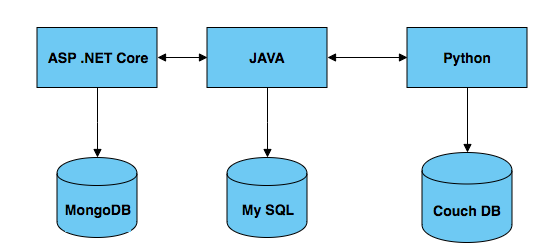
\includegraphics[scale=0.3]{grafiken/microservices.png}
    \caption{ Illustration of services as independent entities \cite{MicroserviceNewMan}}
    \label{fig:serviceExample}
\end{figure}

\par
    Comparing microservices to a single monolithic application where the
    system is built as a large single unit and runs in a single process. 
    This is considered the most natural way to develop a server side 
    application. It is seen that as the application scales in size, it 
    gets harder to keep up with the changes. As scaling requires the whole
    application to be scaled as a whole. This is where microservices come very handy,
    as the only the required bounded module can be scaled up as needed. 
    There are factors to be considered before going for a microservice
    architecture.

    \begin{table}[h!]
        \centering
        \begin{tabular}{|p{9cm}|p{7.5cm}|}
            \hline
                \textbf{Advantages}  & \textbf{Disadvantages}\\
            \hline
                The services can be developed with different languages & 
                A mature team must be present to maintain large number of services \\
            \hline
                A strong modular boundaries is present which reinforces a modular
                structure.
                & All the services must manage eventual consistency which is
                harder to manage in a large distributed system.\\
            \hline
                 Independent deployment is easier since the services are
                 autonomous. & Harder to program since remote calls must be made.\\
            \hline
        \end{tabular}
        \caption{Advantages and disadvantages of microservices \cite{FowlerMartin}}
        \label{table:Advantages and disadvantages of microservices}     
    \end{table}    

    \newpage
    \subsection{Data Sovereignty In Microservice}
    It is an important rule for a microservice architecture to own its domain data and 
    logic. A high cohesion and loose coupling would be an end goal for a microservice.
    It becomes easier to achieve them when 



